%%%%%%%%%%%%%%%%%%%%%%%%%%%%%%%%%%%%%%%%%
% TU Muenchen 17 Sommer Semester
% Applied Reinforcement Learning
% Final Report
%%%%%%%%%%%%%%%%%%%%%%%%%%%%%%%%%%%%%%%%%

%----------------------------------------------------------------------------------------
%	PACKAGES AND OTHER DOCUMENT CONFIGURATIONS
%----------------------------------------------------------------------------------------

\documentclass[a4paper, 11pt]{article} % Font size (can be 10pt, 11pt or 12pt) and paper size (remove a4paper for US letter paper)
%\usepackage{hyperref}

\usepackage[protrusion=true,expansion=true]{microtype} % Better typography
\usepackage{graphicx} % Required for including pictures
\usepackage{wrapfig} % Allows in-line images
\usepackage{booktabs}
\usepackage{mathpazo} % Use the Palatino font
\usepackage[T1]{fontenc} % Required for accented characters
\usepackage{subfigure}
\linespread{1.05} % Change line spacing here, Palatino benefits from a slight increase by default

\makeatletter
\renewcommand\@biblabel[1]{\textbf{#1.}} % Change the square brackets for each bibliography item from '[1]' to '1.'
\renewcommand{\@listI}{\itemsep=0pt} % Reduce the space between items in the itemize and enumerate environments and the bibliography

\renewcommand{\maketitle}{ % Customize the title - do not edit title and author name here, see the TITLE block below
\begin{flushright} % Right align
{\LARGE\@title} % Increase the font size of the title

\vspace{50pt} % Some vertical space between the title and author name

{\large\@author} % Author name
\\\@date % Date

\vspace{40pt} % Some vertical space between the author block and abstract
\end{flushright}
}

%----------------------------------------------------------------------------------------
%	TITLE
%----------------------------------------------------------------------------------------

\title{\textbf{Finding the Shortest Path Using Reinforcement Learning}} % Subtitle

\author{\textsc{Lingfeng Zhang, Wenhan Hao, $\&$ Tianming Qiu} % Author
\\{\textit{}}} % Institution

\date{Group: applied-rl17 / E3} % Date

%----------------------------------------------------------------------------------------

\begin{document}

\maketitle % Print the title section



%----------------------------------------------------------------------------------------
%	ESSAY BODY
%----------------------------------------------------------------------------------------
\section{Introduction}
Reinforcement learning is a powerful framwork for robot to learn novel tasks by
self-practice. Through trial-and-error learning, robotic agent has the chance to
be exploited in a wide range of situations, including industrial and social
applications. In this project, we attempt to employ reinforcement learning for
path planning.
\\[3ex]
Path planning is a basic and widely-studied problem. Also it has many actual
scenarios, for example, autonomous car navigation and drones for logistics.
Typically, a optimal path between two locations on traffic map is computed by
considering both distance and traffic situation. But if prior informantion for
road networks is absent, the planning is essentially impossible. Therefore,
we attempt to empoly reinforcement learning to plan path from scratch.
\\[3ex]
In order to make our project more realistic, we use the map around TUM as the
training map. The original map (left) and the map in simulator (right) are shown
in Figure \ref{fig1}. The simulation map contains several guide lines on the
ground as the roads to form the road network with many crossroads. Two points on
simulation map could be chosen as starting point and destination, and then agent
attempt to discover the optimal path between those two points. In our project,
the e-puck mobile robot takes on a role of explorer.
\begin{figure}[tbp]
\centering
\subfigure[map from google map]{
\label{Fig.sub.1}
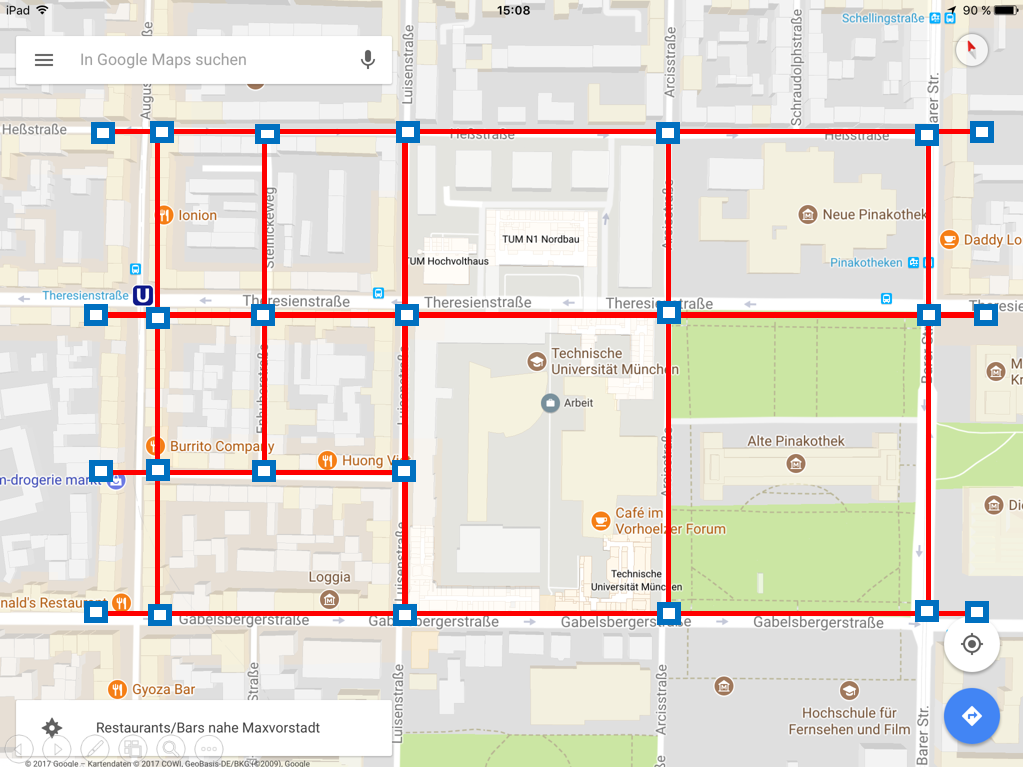
\includegraphics[width=0.45\textwidth]{UniMap.png}}
\subfigure[map in v-rep]{
\label{Fig.sub.2}
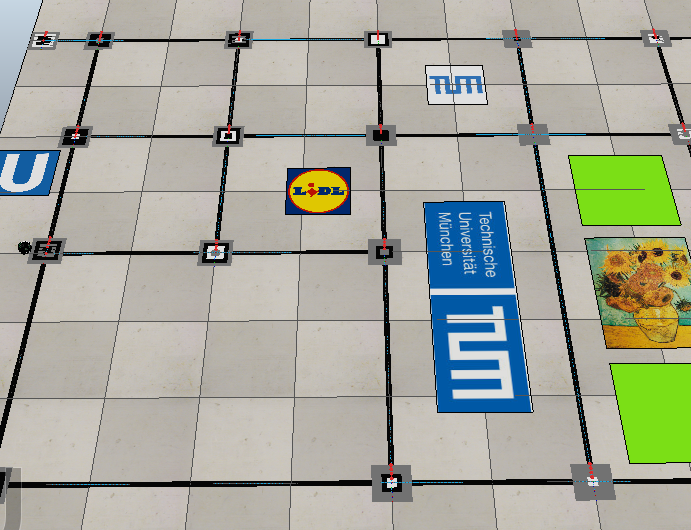
\includegraphics[width=0.45\textwidth]{Vrep2.png}}
\caption{Training maps}
\label{fig1}
\end{figure}


\section{Modeling}
To make our tasks tractable, we consider a grid-based representation with discrete
states and action. The navigational task for our mobile robots could be projected
into this presentation by employing a number of actions such as 'drive east',
'drive west', 'drive north' as well as 'drive south' that only use a low-level
controller that takes care of accelerating, moving, turning and stopping. The
different crossroad in the simulated map will be considered as states. The simulation
map we used has 22 states. In our experiment, we assign a reward '+10' at the destination
state and '-1' at the other states. Also at the blind alley it will get a very poor
reward such as '-10' in order to let agent avoid those states. At the begin of
each simulation, two points will set up as the start point and destination,
and the e-puck robot will be placed in the start point of the training map, and
start to explore the training map. From one state to adjacent state, the robot will
drive along the line we drawn on the ground. The under sensor on e-puck
will scan the ground all the time in order to keep robot following the line
and detect the label we use to distinguish state. Once e-puck reaches the terminal
state(destination), it will be replaced in the same start point and start a new
exploration.

\section{Algorithm}
The reinforcement learning approaches can be categorized into two groups: model-free
method, which directly learns a control policy from system interaction, and
model-based method, which first learn a model of the system dynamics, and then
optimize the policy under this model. At the beginning of our project, we attempt to
set up a model of our environment in order to make learning process more efficient.
We let all transitionprobability be deterministic, i.e, the results of agent performs
an action are deterministic. The results are only depends on current state and performed
action. And then we optimized policy under this policy. But this model is too coarse
and ideal. It doesn't have ability to handle with model uncertainty and complex situation.
As small model errors accumulate, the simulated results can be big different from
real situation. For this reason, we modified our plan, a typical Q-learning algorithm
is used. The agent first observes current state, and then takes action accorading to
policy. After the action is performed, the agent observe a reward and new state.
Then the Q-value is updated by maximizing Q-value of next step.

\section{Milestones}
In the end we have achieved five main Milestones: determination of the mathematical
model, familiar with the software environment, viable physical environment design,
successful implementation of Codes on Vrep, and stably interact with real world.
And there is also a remaining feature: state detection with front camera.
\\[3ex]
First of all, the mathematical model has been determined. Before we
chose the road crossing as states, and we assumed the actions as 'turn right',
'turn left' and so on. However, it caused a serious problem that the model
could not satisfy Markov Property. Assume Epuck comes to a road crossing
several times, first time it comes from north, namely the last state is in the
north direction of current state, and second time comes from south. Since
we treat this road crossing as only one state, if Epuck both choose the action
'turn right', the transition probability of the next state will be totally different
and somehow dependent on not only the current state, but also the state
before, like $P(s_{t+1}|s_t, s_{t-1}, a_t)$. Hence we choose a new set of actions
as 'go east', 'go west', 'go north' and 'go south'. And on the high level of
this problem we just treat our Epuck as a mass point. And leave the detailed
problem of action realizations to the lower level. This approach make sure the
scene satisfies Markov property.
\\[3ex]
Secondly, we learned how to use python and vrep. We don't have any experience on
python before, so we have to learn it from scratch. The interface of vrep is also
a hard problem for us. We spent a lot of time to manipulate it skillfully.
\\[3ex]
Thirdly, a viable simulation map has been designed on Vrep. The
three floor sensors under Epuck are applied to detect the road, and the
road crossings are painted with a three-color barcode in order to distinguish
between different states. Although the floor sensor are not very accurate to
distinguish high resolution color space, it could be sensitive enough to detect
black, white, and gray these three situations. The length of our barcode is 3.
So, it can perform $3^3 = 27$ different states.
\\[3ex]
Next, the simulation execution of Epuck have
been implemented on Vrep by Python. The code can be basically divided
into three main parts: Q-learning algorithm, Motion or action control and
perception part. Q-learning part is designed to select the next action and update
Q-value functions. Motion control is used for the low level control issues such as
'go east', turn a corner and so on. Perception focus on the three floor sensors
to make sure Epuck could follow the line,stop correctly at the crossing roads,
and determine current state.
\\[3ex]
After that, the physical environment is builded, and epuck can stably interact with it.
We printed the map with four sheets of A4 paper. All the states and road are marked
out on the paper. Epuck can distinguish road and different states with the help
of three floor sensors. Three floor sensors scan the ground all thee time in order to
detect the change of colors on the ground.
\\[3ex]
Finally is the still remaining feature: state detection with front camera. State
detection is a key component of our project. At the beginning we attempted to
achieve this feature using front camera. Due to poor resolution and slow transmission
we discarded this plan, and quickly changed to use floor sensor instead.

\section{Conclusion}
After successfully completing this course, we master some basics of reinforcement
learning methods and learn how to model real engineering problems using reinforcement
learning methods. Using this knowledge we constructed and implemented reinforcement
learning algorithms to solve simple robotics problems on the e-Puck platform. And
through practice we are also familiar with python and vrep.






\end{document}
